\documentclass[./main.tex]{subfiles}

\begin{document}

虽然 Haskell 的纯性带来了非常多的便利,但是在处理某些问题时,我们需要不同与命令式语言那样的方式来解决。由于引用透明,Haskell 中相同的值时没有区别的。

如果我们有一颗树的节点都是五,当我们想要将它们其中一个变为六时,我们必须要知道到底究竟是哪个五想要变成六。也就是说必须知道其位置。在不纯的语言中,仅需
知道其内存地址,并改变它。然而在 Haskell 中,一个五跟其它的五并无差异,因此我们不能通过内存地址来进行辨别。同样的,我们也不能真的\textit{修改}任何
东西;当我们说改变一颗树,真正的意思其实是接受一棵树,返回一个与原始树相近的树,且只有细微的不同。

一种方法就是从树的根部记住通向节点的路径,但是这样效率低下。如果想要修改一个临近之前修改过的节点,我们又要从头来过!

本章我们将学习如何集中注意在某个数据结构上,使得改变数据结构与遍历的动作变得高效。

\subsection*{走二元树}

首先是之前章节介绍过的树的定义:

\begin{lstlisting}[language=Haskell]
  data Tree a = Empty | Node a (Tree a) (Tree a) deriving (Show)
\end{lstlisting}

下面是一个数的例子:

\begin{lstlisting}[language=Haskell]
  freeTree :: Tree Char
  freeTree =
    Node
      'P'
      ( Node
          'O'
          (Node 'L' (Node 'N' Empty Empty) (Node 'T' Empty Empty))
          (Node 'Y' (Node 'S' Empty Empty) (Node 'A' Empty Empty))
      )
      ( Node
          'L'
          (Node 'W' (Node 'C' Empty Empty) (Node 'R' Empty Empty))
          (Node 'A' (Node 'A' Empty Empty) (Node 'C' Empty Empty))
      )
\end{lstlisting}

\newpage
其图形如下:

\begin{figure}[h]
  \centering
  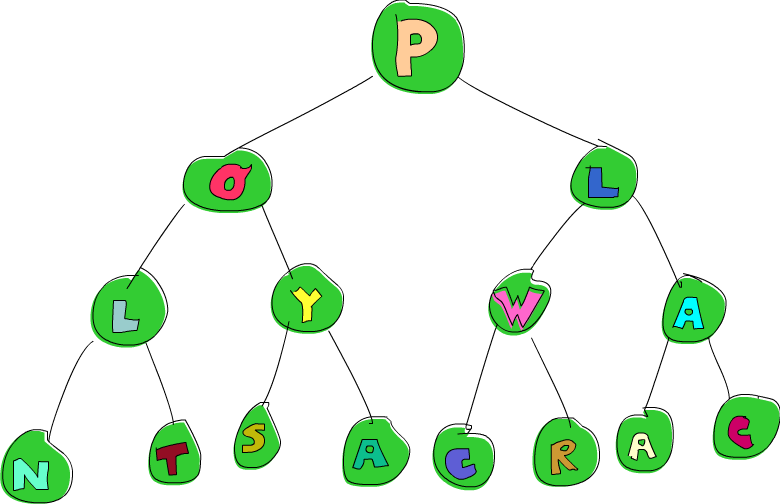
\includegraphics[width=0.8\textwidth]{\subfix{./images/pollywantsa.png}}
\end{figure}

注意到\acode{W}在树中的位置了吗?我们想要将其变为\acode{P}。那么该怎么做呢?其中一种方式就是通过对树进行模式匹配,直到第一次找到该元素的位置,然后再
进行修改:

\begin{lstlisting}[language=Haskell]
  changeTop :: Tree Char -> Tree Char
  changeTop (Node x l (Node y (Node _ m n) r)) = Node x l (Node y (Node 'P' m n) r)
\end{lstlisting}

呃这不仅丑陋而且还令人迷惑。那么发生了什么?首先是模式匹配根元素\acode{x}(即\acode{'P'})以及左子树\acode{l},而对于右子树再次进行模式匹配,以此类推,
最终替换\acode{'W'}成为\acode{'P'}。

那么有没有更好的办法呢?不如构建一个函数,接受一棵树以及一个方向列表。方向即\acode{L}或\acode{R}:

\begin{lstlisting}[language=Haskell]
  data Direction = L | R deriving (Show)

  type Directions = [Direction]

  changeToP :: Directions -> Tree Char -> Tree Char
  changeToP (L : ds) (Node x l r) = Node x (changeToP ds l) r
  changeToP (R : ds) (Node x l r) = Node x l (changeToP ds r)
  changeToP [] (Node _ l r) = Node 'P' l r
\end{lstlisting}

如果方向列表的第一个元素是\acode{L},我们将构建一颗与旧树一样的树,只不过左子树会有元素变为\acode{'P'}。当递归调用\acode{changeToP},则传入列表尾部,
因为头部已经被消费了。\acode{R}同理。如果列表为空,意味着到达了目的地,返回一个新的树,其根被改为\acode{'P'}。

为了避免打印出整棵树,让我们构建一个函数,接受一个方向的列表,返回目的地的元素:

\begin{lstlisting}[language=Haskell]
  elemAt :: Directions -> Tree a -> a
  elemAt (L : ds) (Node _ l _) = elemAt ds l
  elemAt (R : ds) (Node _ _ r) = elemAt ds r
  elemAt [] (Node x _ _) = x
\end{lstlisting}

这个函数跟\acode{changeToP}很像,只不过不是记住路径并重构树,而是忽略所有经过只记住目的地。这里修改了\acode{'W'}至\acode{'P'},检查是否修改成功:

\begin{lstlisting}[language=Haskell]
  ghci> let newTree = changeToP [R,L] freeTree
  ghci> elemAt [R,L] newTree
  'P'
\end{lstlisting}

虽然这个技巧可能看起来很酷,但是它还是低效,特别是当我们需要频繁的修改元素时。假设我们有一个很大的树,一个指向了树底部元素的很长的方向列表。那么当我们修改
一个元素后,又要修改另一个临近的元素,我们又得重头开始一直走到树的底部!

\subsection*{留下面包屑的路径}

那么专注在一个子树,我们希望一个比方向列表更好的东西,避免总是从树的根部开始。那么如果从树根部开始,每次移动一步并留下印记,类似于留下面包屑会有帮助吗?
换言之,向左时记住向左,向右时记住向右。

为了表示面包屑,可以使用一个\acode{Direction}列表,由于我们留下的方向现在是相反的,为了区分\acode{Directions},我们称其为\acode{Breadcrumbs},

\begin{lstlisting}[language=Haskell]
  type Breadcrumbs = [Direction]
\end{lstlisting}

下面是一个接受一棵树以及面包屑的函数,当移动至左子树时,添加\acode{L}在列表头部:

\begin{lstlisting}[language=Haskell]
  goLeft :: (Tree a, Breadcrumbs) -> (Tree a, Breadcrumbs)
  goLeft (Node _ l _, bs) = (l, L : bs)
\end{lstlisting}

忽略根以及右子树,返回左子树以及在旧的面包屑头部添加了\acode{L}的新面包屑。下面是往右的函数:

\begin{lstlisting}[language=Haskell]
  goRight :: (Tree a, Breadcrumbs) -> (Tree a, Breadcrumbs)
  goRight (Node _ _ r, bs) = (r, R : bs)
\end{lstlisting}

现在使用这些函数来接受我们的\acode{freeTree},先是向右再向左:

\begin{lstlisting}[language=Haskell]
  ghci> goLeft (goRight (freeTree, []))
  (Node 'W' (Node 'C' Empty Empty) (Node 'R' Empty Empty),[L,R])
\end{lstlisting}

现在有了一个以\acode{'W'}为根的树,\acode{'C'}为左子树的根而\acode{'R'}为右子树的根,面包屑则为\acode{[L, R]},因为我们是先右后左。

我们可以定义一个\acode{-:}函数来将代码变得更可读:

\begin{lstlisting}[language=Haskell]
  x -: f = f x
\end{lstlisting}

它可以将函数的应用变为先写值,然后是\acode{-:}接着函数。那么改写以后就成了:

\begin{lstlisting}[language=Haskell]
  ghci> (freeTree, []) -: goRight -: goLeft
  (Node 'W' (Node 'C' Empty Empty) (Node 'R' Empty Empty),[L,R])
\end{lstlisting}

\subsubsection*{从后至前}

那么如果想要反向走树呢?根据面包屑我们可以知道当前树是其父树的左子树,然后更上一层则是右子树。仅仅如此,它并没有告知当前子树其父足够的信息,让我们
能够继续往树上走。除了单纯记录方向之外,还必须把其它的数据记录下来。这个案例中就是子树的父信息以及其右子树。

一般而言,一个面包屑有足够的信息用于重建父节点。所以它应该包含所有没有选择的路径信息,记录我们走过的方向;同时它不应该包含现在关注的子树,因为它已经在
元组的第一部分了,如果也记录下来就会有重复的信息。

现在来修改一下面包屑的定义,让它包含我们之前丢掉的信息:

\begin{lstlisting}[language=Haskell]
  data Crumb a = LeftCrumb a (Tree a) | RightCrumb a (Tree a) deriving (Show)
\end{lstlisting}

用\acode{LeftCrumb}来包含我们走过的右子树,以及没走过的右子树,而不是仅仅写个\acode{L},\acode{RightCrumb}同理。

这些面包屑现在包含了重构树所需的所有信息。它们像是软盘一样存储了走过的路径,而不仅仅只有方向。

基本而言可以将每个面包屑视为一个树的节点,树的节点有一个洞,当向树的更深处走,面包屑携带所有走过的信息,除了当前关注的子树被记录在洞那里。

我们也要把\acode{Breadcrumbs}的类型别名改成:

\begin{lstlisting}[language=Haskell]
  type Breadcrumbs' a = [Crumb a]
\end{lstlisting}

接着修改\acode{goLeft}以及\acode{goRight}来记录没有走过的路径信息,而不是像之前那样忽略掉:

\begin{lstlisting}[language=Haskell]
  goLeft' :: (Tree a, Breadcrumbs' a) -> (Tree a, Breadcrumbs' a)
  goLeft' (Node x l r, bs) = (l, LeftCrumb x r : bs)
\end{lstlisting}

类似于之前的\acode{goLeft},不同于仅仅添加一个\acode{L}在面包屑列表头部,而是添加了一个\acode{LeftCrumb}记录从左走过,以及未走过的右子树。

注意该函数假设了当前注意的树并不为\acode{Empty}。一颗空树是不会有任何子树的,所以如果在一颗空树上向左走,异常将会出现,因为对\acode{Node}的
匹配不成功,且没有额外去匹配\acode{Empty}。

\acode{goRight}也类似:

\begin{lstlisting}[language=Haskell]
  goRight' :: (Tree a, Breadcrumbs' a) -> (Tree a, Breadcrumbs' a)
  goRight' (Node x l r, bs) = (r, RightCrumb x l : bs)
\end{lstlisting}

现在有了向左和向右,我们就能具备了返回树根的能力了,以下是\acode{goUp}函数:

\begin{lstlisting}[language=Haskell]
  goUp :: (Tree a, Breadcrumbs' a) -> (Tree a, Breadcrumbs' a)
  goUp (t, LeftCrumb x r : bs) = (Node x t r, bs)
  goUp (t, RightCrumb x l : bs) = (Node x l t, bs)
\end{lstlisting}

该函数接受一个正在关注的树\acode{t},以及一个\acode{Breadcrumbs}用于检查最近的\acode{Crumb},如果是一个\acode{LeftCrumb},那么构建一颗新树,
而\acode{t}作为该树的左子树。这里通过两次模式匹配,首先是\acode{Breadcrumbs}的头,接着是\acode{LeftCrumb},拿到\acode{x}右子树\acode{r}
用来构建\acode{Node}剩余部分,并将剩下的\acode{Breadcrumbs}即\acode{bs}一并返回。

注意该函数在树的顶部会导致错误,稍后我们将用\acode{Maybe}单子来代表失败来进行改进。

有了一对元组\acode{Tree a}与\acode{Breadcrumbs a},我们便具备了所有重构的信息。这个模版可以让向上,向左以及向右变得简单很多。这样一对包含了关注的
部分以及其它信息的元组被称为 zipper。因此我们可以对其进行类型别名:

\begin{lstlisting}[language=Haskell]
  type Zipper a = (Tree a, Breadcrumbs' a)
\end{lstlisting}

\subsubsection*{操作当前注意的树}

现在我们有了向上与向下的移动,那么就可以构建一个函数用于修改 zipper 所关注的元素了:

\begin{lstlisting}[language=Haskell]
  modify :: (a -> a) -> Zipper a -> Zipper a
  modify f (Node x l r, bs) = (Node (f x) l r, bs)
  modify f (Empty, bs) = (Empty, bs)
\end{lstlisting}

如果关注在一个节点,通过函数\acode{f}修改其根元素;如果关注在一颗空树,则不做改动。测试:

\begin{lstlisting}[language=Haskell]
  ghci> let newFocus = modify (\_ -> 'P') (goRight (goLeft (freeTree,[])))
\end{lstlisting}

用可读性更好的\acode{-:}函数:

\begin{lstlisting}[language=Haskell]
  ghci> let newFocus = (freeTree,[]) -: goLeft -: goRight -: modify (\_ -> 'P')
\end{lstlisting}

接着是向上移动,替换字符为\acode{'X'}:

\begin{lstlisting}[language=Haskell]
  ghci> let newFocus2 = modify (\_ -> 'X') (goUp newFocus)
\end{lstlisting}

使用\acode{-:}:

\begin{lstlisting}[language=Haskell]
  ghci> let newFocus2 = newFocus -: goUp -: modify (\_ -> 'X')
\end{lstlisting}

向上移动很简单,因为面包屑的另一部分数据结构是没有关注的,不过它是倒转过来的,有点像是要把袜子反过来才能用那样。有了这些信息,我们便不用再从根走一遍,
而是从反过来的树顶部开始,将其部分翻转后再将其置为关注。

每个节点都有两个子树,即使这些子树是空树。所以当关注了一颗空的子树,可以将其替换为一颗非空子树,即叶节点:

\begin{lstlisting}[language=Haskell]
  attach :: Tree a -> Zipper a -> Zipper a
  attach t (_, bs) = (t, bs)
\end{lstlisting}

接受一颗树以及一个 zipper 并返回一个新的 zipper,其关注的被替换为接受的树。我们不仅能用这个方法来延展一棵树,还可以替换整个子树。通过\acode{attach}
来替换\acode{freeTree}最左的树:

\begin{lstlisting}[language=Haskell]
  ghci> let farLeft = (freeTree,[]) -: goLeft -: goLeft -: goLeft -: goLeft
  ghci> let newFocus = farLeft -: attach (Node 'Z' Empty Empty)
\end{lstlisting}

\subsubsection*{直接走到树顶端}

直接走到树顶端很简单:

\begin{lstlisting}[language=Haskell]
  topMost :: Zipper a -> Zipper a
  topMost (t,[]) = (t,[])
  topMost z = topMost (goUp z)
\end{lstlisting}

如果面包屑没了,那么就表示已经在树的根处了,并返回当前关注的树。

\subsection*{专注于列表}

Zippers 几乎可以用于任何数据结构,不出意外它可以被用于列表的列表。毕竟列表很像树,只不过在树中的节点有若干子树,而列表中的节点只包含一个子列表。我们在
定义自己的列表类型那一章中,定义了如下数据类型:

\begin{lstlisting}[language=Haskell]
  data List a = Empty | Cons a (List a) deriving (Show, Read, Eq, Ord)
\end{lstlisting}

现在让我们为列表做一个 zipper。切换子列表关注,我们只需要向前或者向后移动(不同于树的向上,向左或向右)。在树的情景下,关注的部分是一颗子树,另外还携带
就是移动后的面包屑。那么对于列表而言,单个面包屑应该由什么构成呢?在处理二元树时,面包屑必须包含父节点的根以及其它没有走过的子树,同时还要记住左右方向。
因此它必须包含一个节点的所有信息,除了正在关注子树(存于 zipper 的第一部分)。

列表比数简单多了,无需记住左右方向,因为只有一个方向即深入列表。又因为每个节点仅有一颗子树,也无需记住没有走过的路径。这么看上去只需要记住上一个元素即可。
假设有一个列表\acode{[3,4,5]}且已知上一个元素是\acode{2},那么可以将其放置在列表头部,得\acode{[2,3,4,5]}。

由于单个面包屑在这里仅为一个元素,我们无需将其置入一个数据类型,比如为树所创建的\acode{Crumb}数据类型那样,只需要类型别名即可:

\begin{lstlisting}[language=Haskell]
  type ListZipper a = ([a], [a])
\end{lstlisting}

这里第一个列表代表正在关注着的列表,而第二个列表则是面包屑列表。下面是向前与向后的函数:

\begin{lstlisting}[language=Haskell]
  goForward :: ListZipper a -> ListZipper a
  goForward (x : xs, bs) = (xs, x : bs)

  goBack :: ListZipper a -> ListZipper a
  goBack (xs, b : bs) = (b : xs, bs)
\end{lstlisting}

当向前时,我们关注当前列表的尾部并留下头部元素作为一个面包屑;当向后时,我们获取最近的面包屑并将其置入关注列表的头部。

测试:

\begin{lstlisting}[language=Haskell]
  ghci> let xs = [1,2,3,4]
  ghci> goForward (xs,[])
  ([2,3,4],[1])
  ghci> goForward ([2,3,4],[1])
  ([3,4],[2,1])
  ghci> goForward ([3,4],[2,1])
  ([4],[3,2,1])
  ghci> goBack ([4],[3,2,1])
  ([3,4],[2,1])
\end{lstlisting}

可以看到面包屑在列表的情况下就是一个倒转的列表。移出的元素进入面包屑的头部,因此移动回去只需将面包屑的头部元素移动进关注列表。

这也是为什么称其为一个拉链 zipper,因为这看上去就像是拉链上下移动。

\subsection*{一个简单的文件系统}

理解了 zipper 是如何运作的,现在让我们用树来表达一个简单的文件一同,接着为其构建一个 zipper,使得我们可以在文件夹之间移动,就像是我们通常使用文件系统
进行跳转那样。

简单的来看一个文件系统,基本上就是由文件与文件夹构成。以下是一些类型别名以及一个数据类型:

\begin{lstlisting}[language=Haskell]
  type Name = String
  type Data = String
  data FSItem = File Name Data | Folder Name [FSItem] deriving (Show)
\end{lstlisting}

文件包含了两个字符串,前者为名称,后者为数据。文件夹包含了一个字符串以及一个列表的文件系统,如果列表为空则意为空文件夹。

以下是一个包含了文件和子文件夹的文件夹:

\begin{lstlisting}[language=Haskell]
  myDisk :: FSItem
  myDisk =
    Folder
      "root"
      [ File "goat_yelling_like_man.wmv" "baaaaaa",
        File "pope_time.avi" "god bless",
        Folder
          "pics"
          [ File "ape_throwing_up.jpg" "bleargh",
            File "watermelon_smash.gif" "smash!!",
            File "skull_man(scary).bmp" "Yikes!"
          ],
        File "dijon_poupon.doc" "best mustard",
        Folder
          "programs"
          [ File "fartwizard.exe" "10gotofart",
            File "owl_bandit.dmg" "mov eax, h00t",
            File "not_a_virus.exe" "really not a virus",
            Folder
              "source code"
              [ File "best_hs_prog.hs" "main = print (fix error)",
                File "random.hs" "main = print 4"
              ]
          ]
      ]
\end{lstlisting}

\subsubsection*{文件系统的 zipper}

我们有了一个文件系统,我们需要一个 zipper 是我们可以走动,增加,修改,或者移除文件或文件夹。像是二元树或列表那样,用面包屑来保存走过路径的信息。一个面包屑
就是一个节点,它包含了除了正在关注的子树之外的所有信息。

在此,一个面包屑应该像是一个文件夹,它无需包含当前关注的文件夹。你可能会问为什么不是一个文件呢?因为如果关注在一个文件,我们就无法深入文件系统,因此留下一个
从文件而来的面包屑没有意义。一个文件就类似于一颗空树。

如果关注在\acode{"root"}文件夹,接着将关注转到文件\acode{"dijon_poupon.doc"},那么这个时候的面包屑应该长什么样?它应该包含了父文件夹的名称,以及这个
文件之前以及之后的所有项。通过两个独立的列表分别保存之前的项与之后的项,我们可以精确的知道回去时的地址。

下面是面包屑的类型:

\begin{lstlisting}[language=Haskell]
  data FSCrumb = FSCrumb Name [FSItem] [FSItem] deriving (Show)
\end{lstlisting}

以及 zipper 的类型别名:

\begin{lstlisting}[language=Haskell]
  type FSZipper = (FSItem, [FSCrumb])
\end{lstlisting}

返回父节点非常的容易,仅需将最近的面包屑与当前所关注的进行组合:

\begin{lstlisting}[language=Haskell]
  fsUp :: FSZipper -> FSZipper
  fsUp (item, FSCrumb name ls rs : bs) = (Folder name (ls ++ [item] ++ rs), bs)
\end{lstlisting}

因为面包屑知道父文件夹的名称,以及所关注项之前(\acode{ls})与之后(\acode{rs})的所有项,所以移动就很简单了。

那么更深入文件系统呢?假设从\acode{"root"}到\acode{"dijon_poupon.doc"},那么面包屑就包含了\acode{"root"},以及在\acode{"dijon_poupon.doc"}
之前的所有项以及之后的所有项。

下面是一个函数,接受一个名称,并关注在当前文件夹下的一个文件或文件夹:

\begin{lstlisting}[language=Haskell]
  fsTo :: Name -> FSZipper -> FSZipper
  fsTo name (Folder folderName items, bs) =
    let (ls, item : rs) = break (nameIs name) items
     in (item, FSCrumb folderName ls rs : bs)

  nameIs :: Name -> FSItem -> Bool
  nameIs name (Folder folderName _) = name == folderName
  nameIs name (File fileName _) = name == fileName
\end{lstlisting}

\acode{fsTo}接受一个\acode{Name}与一个\acode{FSZipper}并返回一个新的\acode{FSZipper},其关注移至给定名称。该文件必须处于当前所关注的文件夹下。

这里首先用了\acode{break}来将列表分成前后两个列表。\acode{break}函数接受一个子句以及一个列表,返回两个列表,前者为不满足子句的所有项所组成的列表,
而后者为第一个满足子句的项以及该项之后的所有项所组成的列表。

那么在此,\acode{ls}就是一个在查询项之前的所有项,\acode{item}就是查询的项,而\acode{rs}则是\acode{item}后的所有项。有了这些,从\acode{break}
所得到的项作为关注项,并构建一个面包屑。

注意如果所查询的项并非一个文件夹,模式\acode{item:rs}则会尝试匹配一个空列表,继而报错。同理,如果当前关注的并非一个文件夹而是一个文件时,我们也会得到
报错使得程序崩溃。

现在可以对文件系统进行上下移动了。首先从根开始,再走到\acode{"skull_man(scary).bmp"}文件那儿。

\begin{lstlisting}[language=Haskell]
  let newFocus = (myDisk, []) -: fsTo "pics" -: fsTo "skull_man(scary).bmp"
\end{lstlisting}

\acode{newFocus}现在是一个 zipper,其关注在\acode{"skull_man(scary).bmp"}文件上。现在让我们看看它是否正确:

\begin{lstlisting}[language=Haskell]
  ghci> fst newFocus
  File "skull_man(scary).bmp" "Yikes!"
\end{lstlisting}

接着向上移动接着关注到相邻文件\acode{"watermelon_smash.gif"}:

\begin{lstlisting}[language=Haskell]
  ghci> let newFocus2 = newFocus -: fsUp -: fsTo "watermelon_smash.gif"
  ghci> fst newFocus2
  File "watermelon_smash.gif" "smash!!"
\end{lstlisting}

\subsubsection*{操作文件系统}

我们现在知道了该如何在文件系统中移动,操作它们也很简单。以下函数用于对当前关注的文件或文件夹进行改名:

\begin{lstlisting}[language=Haskell]
  fsRename :: Name -> FSZipper -> FSZipper
  fsRename newName (Folder name items, bs) = (Folder newName items, bs)
  fsRename newName (File name dat, bs) = (File newName dat, bs)
\end{lstlisting}

将\acode{"pics"}文件夹改名为\acode{"cspi"}:

\begin{lstlisting}[language=Haskell]
  ghci> let newFocus = (myDisk,[]) -: fsTo "pics" -: fsRename "cspi" -: fsUp
\end{lstlisting}

接下来是创建新文件:

\begin{lstlisting}[language=Haskell]
  fsNewFile :: FSItem -> FSZipper -> FSZipper
  fsNewFile item (Folder folderName items, bs) = (Folder folderName (item : items), bs)
\end{lstlisting}

让我们在\acode{"pics"}文件夹下创建一个新文件,然后再移动回跟目录:

\begin{lstlisting}[language=Haskell]
  ghci> let newFocus = (myDisk,[]) -: fsTo "pics" -: fsNewFile (File "heh.jpg" "lol") -: fsUp
\end{lstlisting}

这里很酷的一点就是当我们在修改文件系统时,它并没有真正的被修改,而是返回了一个新的文件系统。这样我们就可以访问我们旧的文件系统(即\acode{myDisk}),
同时可以通过 zipper 访问新的系统(\acode{newFocus}的第一个部分),这样就自动获得了版本控制。这并不仅限于 zippers,而是 Haskell 的数据结构是
不可变的特性。有了 zippers 我们可以更加轻松且有效率的处理数据结构,也因此 Haskell 数据结构的持久性才真正开始闪耀。

\subsection*{注意你的脚步}

迄今如此,当走过数据结构时,无论是二元树,列表还是文件系统,我们并没有关心走了几步。例如\acode{goLeft}函数接受一个二元树的 zipper,接着将关注移动
至子树:

\begin{lstlisting}[language=Haskell]
  goLeft :: Zipper a -> Zipper a
  goLeft (Node x l r, bs) = (l, LeftCrumb x r:bs)
\end{lstlisting}

如果我们走到了一个空树会如何呢?也就是说不是一个\acode{Node},而是一个\acode{Empty}。这种情况下我们会得到一个运行时错误,因为模式匹配将失败,
同时我们没有为空树设计匹配。

让我们使用\acode{Maybe}单子来为我们的移动添加一个可能失败的 context。

\begin{lstlisting}[language=Haskell]
  goLeft :: Zipper a -> Maybe (Zipper a)
  goLeft (Node x l r, bs) = Just (l, LeftCrumb x r : bs)
  goLeft (Empty, _) = Nothing

  goRight :: Zipper a -> Maybe (Zipper a)
  goRight (Node x l r, bs) = Just (r, RightCrumb x l : bs)
  goRight (Empty, _) = Nothing
\end{lstlisting}

测试:

\begin{lstlisting}[language=Haskell]
  ghci> goLeft (Empty, [])
  Nothing
  ghci> goLeft (Node 'A' Empty Empty, [])
  Just (Empty,[LeftCrumb 'A' Empty])
\end{lstlisting}

那么向上呢?

\begin{lstlisting}[language=Haskell]
  goUp :: Zipper a -> Maybe (Zipper a)
  goUp (t, LeftCrumb x r : bs) = Just (Node x t r, bs)
  goUp (t, RightCrumb x l : bs) = Just (Node x l t, bs)
  goUp (_, []) = Nothing
\end{lstlisting}

测试:

\begin{lstlisting}[language=Haskell]
  gchi> let newFocus = (freeTree,[]) -: goLeft -: goRight
\end{lstlisting}

由于现在返回的是\acode{Maybe (Zipper a)}而不是\acode{Zipper a},那么链式函数的方法就不管用了。不过我们可以使用\acode{>>=}来解决这个问题。

\begin{lstlisting}[language=Haskell]
  ghci> let coolTree = Node 1 Empty (Node 3 Empty Empty)
  ghci> return (coolTree,[]) >>= goRight
  Just (Node 3 Empty Empty,[RightCrumb 1 Empty])
  ghci> return (coolTree,[]) >>= goRight >>= goRight
  Just (Empty,[RightCrumb 3 Empty,RightCrumb 1 Empty])
  ghci> return (coolTree,[]) >>= goRight >>= goRight >>= goRight
  Nothing
\end{lstlisting}

\end{document}
